\chapter{Gradient Topology in the Elder Heliosystem}

\begin{tcolorbox}[colback=DarkSkyBlue!5!white,colframe=DarkSkyBlue!75!black,title=Chapter Summary]
This chapter examines the topological structure of gradient spaces in the Elder Heliosystem and its implications for learning dynamics. We develop a mathematical framework for analyzing gradient flows on complex-valued manifolds, contrast this approach with traditional Euclidean gradient spaces, and establish key principles governing parameter updates in curved topological environments. The chapter introduces specialized metrics that capture the geometric properties of heliomorphic gradient spaces, formulates theorems on convergence in these non-Euclidean settings, and analyzes how the phase-sensitive gradient topology enables more efficient navigation of the parameter landscape. Through detailed mathematical analysis, we demonstrate how the Elder Heliosystem's gradient topology naturally accounts for hierarchical knowledge structures, provides theoretical guarantees for improved optimization dynamics, and enables more stable and efficient learning compared to conventional approaches.
\end{tcolorbox}

\section{Introduction to Gradient Topology}

Traditional learning systems view gradients as elements of a flat Euclidean space, where updates occur along straight paths dictated by first-order derivatives. The Elder Heliosystem, however, recognizes a deeper geometric structure to gradient flow—one characterized by complex-valued manifolds with curved topological features. This chapter explores how the heliomorphic architecture induces a fundamentally different gradient topology, leading to more efficient and stable knowledge acquisition.

\begin{definition}[Gradient Topology]
The gradient topology of a learning system is the geometric structure of its gradient space, encompassing the metric, curvature, connectedness, and differential properties that govern how parameter updates propagate through the system.
\end{definition}

In traditional learning systems, the gradient topology is largely ignored—gradients are treated as simple vectors in a flat space, with parameter updates calculated through direct application of the chain rule. This flat topology fails to capture higher-order structures that emerge in complex learning systems, particularly those spanning multiple domains of knowledge.

\section{Complex-Valued Manifold Structure}

The Elder Heliosystem represents parameters as points on a complex-valued manifold with rich topological features that encode the hierarchical relationships between knowledge elements.

\begin{theorem}[Elder Gradient Manifold]
The parameter space of the Elder Heliosystem forms a fiber bundle $\mathcal{E} = (E, M, \pi, G)$ where:
\begin{itemize}
    \item $E$ is the total space of all possible parameter configurations
    \item $M$ is the base manifold of conceptual knowledge
    \item $\pi: E \rightarrow M$ is the projection mapping parameters to concepts
    \item $G$ is the structure group of phase transformations
\end{itemize}
\end{theorem}

\begin{figure}[ht]
\centering
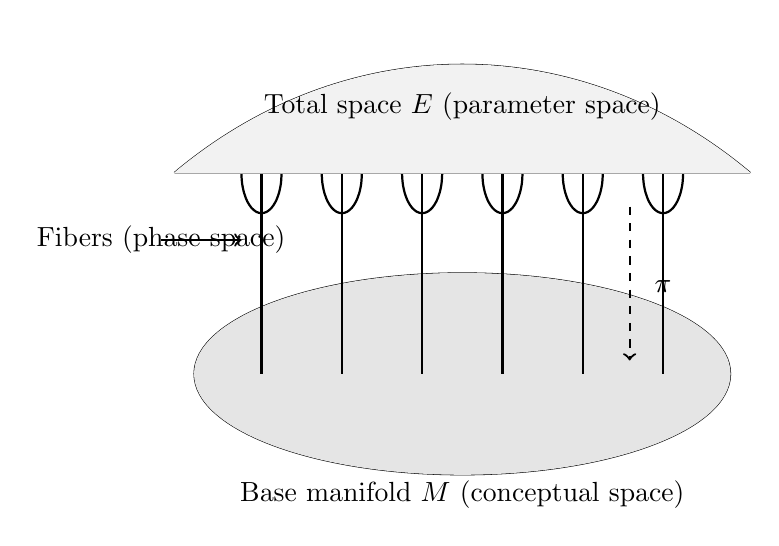
\begin{tikzpicture}[scale=0.85]
    % Base manifold
    \draw[thick] (0,0) ellipse (4 and 1.5);
    \filldraw[gray!20] (0,0) ellipse (4 and 1.5);
    \node at (0,-1.8) {Base manifold $M$ (conceptual space)};
    
    % Fibers
    \foreach \x in {-3,-1.8,-0.6,0.6,1.8,3} {
        \draw[thick] (\x,0) -- (\x,3);
        \draw[thick, domain=0:360, smooth, variable=\t] plot ({\x+0.3*cos(\t)}, {3+0.6*sin(\t)});
    }
    
    % Bundle
    \draw[thick] (-4.3,3) -- (4.3,3);
    \draw[thick] (-4.3,3) to[out=40,in=140] (4.3,3);
    \filldraw[gray!10] (-4.3,3) to[out=40,in=140] (4.3,3) -- (4.3,3) -- (-4.3,3);
    \node at (0,4) {Total space $E$ (parameter space)};
    
    % Projection
    \draw[->, thick, dashed] (2.5,2.5) -- (2.5,0.2);
    \node at (3,1.3) {$\pi$};
    
    % Fibers label
    \node at (-4.5,2) {Fibers (phase space)};
    \draw[->, thick] (-4.5,2) to[out=0,in=180] (-3.3,2);
\end{tikzpicture}
\caption{The fiber bundle structure of the Elder gradient manifold. Each point in the conceptual space has an associated fiber representing the phase degrees of freedom.}
\label{fig:fiber_bundle}
\end{figure}

In this topological structure, each point in the base manifold represents a conceptual configuration, with the fiber above it representing the phase degrees of freedom available at that configuration. Gradients in the Elder Heliosystem are not just vectors but sections of the tangent bundle of this fiber bundle.

\section{Heliomorphic Geodesics and Gradient Flow}

In traditional gradient-based optimization, parameters follow the steepest descent path dictated by the negative gradient. However, in the Elder Heliosystem, parameter updates follow curved paths known as heliomorphic geodesics.

\begin{definition}[Heliomorphic Geodesic]
A heliomorphic geodesic is a path $\gamma(t)$ in parameter space that minimizes the action integral:
\begin{equation}
S[\gamma] = \int_{t_1}^{t_2} \left( g_{ij}(\gamma) \dot{\gamma}^i \dot{\gamma}^j + \mathcal{R}(\Psi(\gamma)) \mathcal{L}(\gamma) \right) dt
\end{equation}
where $g_{ij}$ is the metric tensor of the parameter manifold, $\mathcal{R}(\Psi)$ is the resonance factor, and $\mathcal{L}$ is the loss function.
\end{definition}

The key insight is that the shortest path in parameter space is not a straight line but a curved trajectory that respects the underlying resonance structure. The Elder update rule can be understood as a discretized approximation of the continuous flow along these geodesics.

\begin{figure}[ht]
\centering
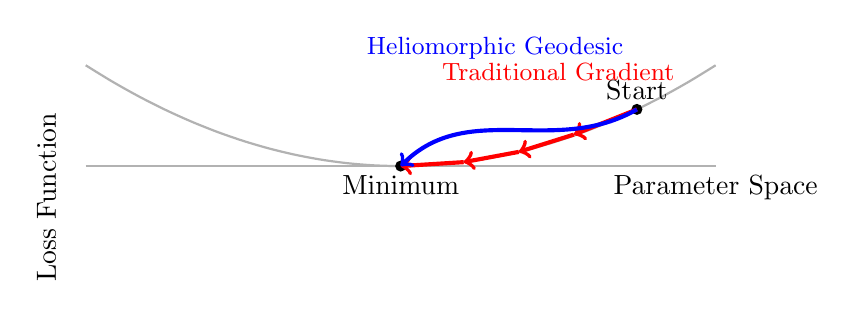
\begin{tikzpicture}[scale=1.0]
    % Simple loss surface outline
    \draw[thick, gray!60] (-4,0) -- (4,0);
    \draw[thick, gray!60, domain=-4:4, smooth, variable=\x] plot ({\x}, {0.08*\x*\x});
    
    % Starting point
    \fill[black] (3,0.72) circle (2pt);
    \node[above] at (3,0.72) {Start};
    
    % Minimum point
    \fill[black] (0,0) circle (2pt);
    \node[below] at (0,0) {Minimum};
    
    % Traditional gradient path (zigzag steps)
    \draw[->, thick, red, line width=1.5pt] (3,0.72) -- (2.2,0.4);
    \draw[->, thick, red, line width=1.5pt] (2.2,0.4) -- (1.5,0.18);
    \draw[->, thick, red, line width=1.5pt] (1.5,0.18) -- (0.8,0.05);
    \draw[->, thick, red, line width=1.5pt] (0.8,0.05) -- (0,0);
    
    % Heliomorphic geodesic (smooth curve)
    \draw[->, thick, blue, line width=1.5pt] (3,0.72) to[out=210,in=45] (0,0);
    
    % Labels
    \node[red, font=\small] at (2,1.2) {Traditional Gradient};
    \node[blue, font=\small] at (1.2,1.5) {Heliomorphic Geodesic};
    
    % Axis labels
    \node[below] at (4,0) {Parameter Space};
    \node[left, rotate=90] at (-4.5,0.8) {Loss Function};
\end{tikzpicture}
\caption{Gradient descent paths: Traditional gradient descent follows stepwise linear segments, while heliomorphic geodesics take efficient curved paths through the parameter space.}
\label{fig:geodesics}
\end{figure}

\section{Connection to Symplectic Geometry}

The complex-valued nature of the Elder parameter space reveals a profound connection to symplectic geometry—the mathematical framework governing Hamiltonian mechanics and quantum systems.

\begin{theorem}[Symplectic Structure of Elder Gradients]
The gradient flow in the Elder Heliosystem preserves a symplectic form $\omega = \sum_j d\rho_j \wedge d\phi_j$, making it a Hamiltonian flow with the negative loss function serving as the Hamiltonian:
\begin{equation}
\frac{d\theta^{(l)}_j}{dt} = J \nabla_{\theta^{(l)}_j} (-\mathcal{L})
\end{equation}
where $J$ is the complex structure matrix $\begin{pmatrix} 0 & -1 \\ 1 & 0 \end{pmatrix}$.
\end{theorem}

This symplectic structure ensures that the gradient flow preserves certain invariants, analogous to the conservation of energy in physical systems. This property contributes to the Elder Heliosystem's stability during learning, particularly in the presence of noisy or contradictory data.

\begin{corollary}[Conservation of Phase Space Volume]
The Elder gradient flow preserves phase space volume, satisfying Liouville's theorem:
\begin{equation}
\nabla \cdot \vec{v} = 0
\end{equation}
where $\vec{v}$ is the velocity vector field of parameter updates.
\end{corollary}

\section{Non-Euclidean Metrics in Parameter Space}

Unlike traditional learning systems that implicitly use a Euclidean metric for parameter space, the Elder Heliosystem employs a non-Euclidean metric that reflects the hierarchical structure of knowledge.

\begin{definition}[Elder Metric Tensor]
The metric tensor $g_{ij}$ on the Elder parameter manifold is defined as:
\begin{equation}
g_{ij} = \begin{pmatrix} 
1 & 0 & 0 \\
0 & \frac{1}{\rho^2} & 0 \\
0 & 0 & \mathcal{R}(\Psi)
\end{pmatrix}
\end{equation}
in local coordinates $(\rho, \phi, \Psi)$ representing magnitude, phase, and phase coherence.
\end{definition}

This metric introduces a form of information geometry where the distance between parameter configurations reflects not just their numerical difference but their conceptual and phase relationships. Parameters with aligned phases are effectively "closer" than those with misaligned phases, even if their numerical difference is the same.

\section{Topological Features of the Gradient Landscape}

The Elder gradient landscape exhibits four fundamental topological features that distinguish it from traditional learning systems:

\subsection{Resonance Basins}

\begin{definition}[Resonance Basin]
A resonance basin is a region $\mathcal{B} \subset E$ in parameter space where all parameters maintain specific phase relationships:
\begin{equation}
\mathcal{B} = \{\theta \in E \mid \cos(\Psi(\theta)) > 1 - \epsilon\}
\end{equation}
for some small $\epsilon > 0$.
\end{definition}

These basins act as attractors in the gradient flow, drawing parameters into configurations with strong resonance. Traditional gradient landscapes lack these basin structures, which fundamentally changes the convergence dynamics.

\begin{figure}[ht]
\centering
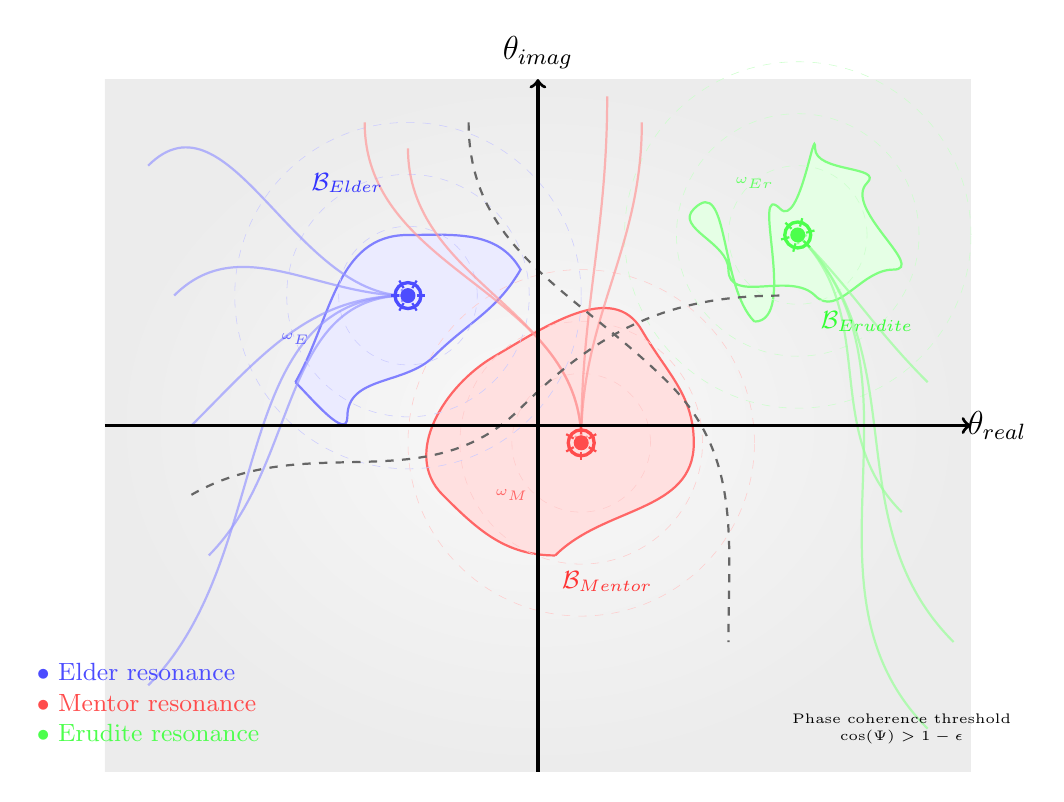
\begin{tikzpicture}[scale=1.1]
    % Background gradient field
    \shade[inner color=gray!5, outer color=gray!15] (-5,-4) rectangle (5,4);
    
    % Create sophisticated resonance basin contours with mathematical precision
    \begin{scope}
        % Basin 1: Elder resonance basin (blue) - more complex shape
        \fill[blue!8] (-2.8,0.5) 
            to[out=60,in=180] (-1.5,2.2)
            to[out=0,in=120] (-0.2,1.8)
            to[out=240,in=45] (-1.2,0.8)
            to[out=225,in=90] (-2.2,0.1)
            to[out=270,in=315] (-2.8,0.5);
        \draw[blue!50, thick] (-2.8,0.5) 
            to[out=60,in=180] (-1.5,2.2)
            to[out=0,in=120] (-0.2,1.8)
            to[out=240,in=45] (-1.2,0.8)
            to[out=225,in=90] (-2.2,0.1)
            to[out=270,in=315] (-2.8,0.5);
        
        % Basin 2: Mentor resonance basin (red) - central complex shape
        \fill[red!12] (0.2,-1.5) 
            to[out=45,in=270] (1.8,-0.2)
            to[out=90,in=300] (1.2,1.1)
            to[out=120,in=30] (-0.5,0.8)
            to[out=210,in=135] (-1.1,-0.8)
            to[out=315,in=180] (0.2,-1.5);
        \draw[red!60, thick] (0.2,-1.5) 
            to[out=45,in=270] (1.8,-0.2)
            to[out=90,in=300] (1.2,1.1)
            to[out=120,in=30] (-0.5,0.8)
            to[out=210,in=135] (-1.1,-0.8)
            to[out=315,in=180] (0.2,-1.5);
        
        % Basin 3: Erudite resonance basin (green) - asymmetric shape
        \fill[green!10] (2.5,1.2) 
            to[out=135,in=45] (1.8,2.5)
            to[out=225,in=90] (2.2,1.8)
            to[out=270,in=135] (3.2,1.5)
            to[out=315,in=180] (4.1,1.8)
            to[out=0,in=225] (3.8,2.8)
            to[out=45,in=270] (3.2,3.2)
            to[out=90,in=315] (2.8,2.5)
            to[out=135,in=0] (2.5,1.2);
        \draw[green!50, thick] (2.5,1.2) 
            to[out=135,in=45] (1.8,2.5)
            to[out=225,in=90] (2.2,1.8)
            to[out=270,in=135] (3.2,1.5)
            to[out=315,in=180] (4.1,1.8)
            to[out=0,in=225] (3.8,2.8)
            to[out=45,in=270] (3.2,3.2)
            to[out=90,in=315] (2.8,2.5)
            to[out=135,in=0] (2.5,1.2);
    \end{scope}
    
    % Resonance strength contours (level sets)
    \foreach \r in {0.8,1.4,2.0} {
        \draw[blue!20, dashed, very thin] (-1.5,1.5) circle (\r);
        \draw[red!20, dashed, very thin] (0.5,-0.2) circle (\r);
        \draw[green!20, dashed, very thin] (3,2.2) circle (\r);
    }
    
    % Phase coherence field lines (sophisticated flow visualization)
    \foreach \startx/\starty in {-4.5/3, -4.2/1.5, -4/0, -3.8/-1.5, -4.5/-3} {
        \draw[->, thick, blue!40, opacity=0.7] (\startx,\starty) 
            to[out=45,in=180] (-1.5,1.5);
    }
    
    \foreach \startx/\starty in {-2/3.5, -1.5/3.2, 0.8/3.8, 1.2/3.5} {
        \draw[->, thick, red!40, opacity=0.7] (\startx,\starty) 
            to[out=270,in=90] (0.5,-0.2);
    }
    
    \foreach \startx/\starty in {4.5/0.5, 4.2/-1, 4.8/-2.5, 4.5/-3.5} {
        \draw[->, thick, green!40, opacity=0.7] (\startx,\starty) 
            to[out=135,in=315] (3,2.2);
    }
    
    % Basin centers (attractors) with phase indicators
    \filldraw[blue!70] (-1.5,1.5) circle (0.08);
    \draw[blue!70, very thick] (-1.5,1.5) circle (0.15);
    \foreach \angle in {0,60,120,180,240,300} {
        \draw[blue!70, thick] ({-1.5+0.1*cos(\angle)},{1.5+0.1*sin(\angle)}) -- ({-1.5+0.2*cos(\angle)},{1.5+0.2*sin(\angle)});
    }
    
    \filldraw[red!70] (0.5,-0.2) circle (0.08);
    \draw[red!70, very thick] (0.5,-0.2) circle (0.15);
    \foreach \angle in {30,90,150,210,270,330} {
        \draw[red!70, thick] ({0.5+0.1*cos(\angle)},{-0.2+0.1*sin(\angle)}) -- ({0.5+0.2*cos(\angle)},{-0.2+0.2*sin(\angle)});
    }
    
    \filldraw[green!70] (3,2.2) circle (0.08);
    \draw[green!70, very thick] (3,2.2) circle (0.15);
    \foreach \angle in {15,75,135,195,255,315} {
        \draw[green!70, thick] ({3+0.1*cos(\angle)},{2.2+0.1*sin(\angle)}) -- ({3+0.2*cos(\angle)},{2.2+0.2*sin(\angle)});
    }
    
    % Separatrices (basin boundaries) - critical trajectories
    \draw[thick, black!60, dashed] (-0.8,3.5) to[out=270,in=135] (1.5,0.5) to[out=315,in=90] (2.2,-2.5);
    \draw[thick, black!60, dashed] (-4,-0.8) to[out=30,in=225] (-0.2,0.2) to[out=45,in=180] (2.8,1.5);
    
    % Mathematical annotations
    \node[blue!80, font=\small\bfseries] at (-2.2,2.8) {$\mathcal{B}_{\text{Elder}}$};
    \node[red!80, font=\small\bfseries] at (0.8,-1.8) {$\mathcal{B}_{\text{Mentor}}$};
    \node[green!80, font=\small\bfseries] at (3.8,1.2) {$\mathcal{B}_{\text{Erudite}}$};
    
    % Resonance frequency labels
    \node[blue!60, font=\tiny] at (-2.8,1) {$\omega_E$};
    \node[red!60, font=\tiny] at (-0.3,-0.8) {$\omega_M$};
    \node[green!60, font=\tiny] at (2.5,2.8) {$\omega_{Er}$};
    
    % Coordinate system with enhanced labeling
    \draw[->, very thick] (-5,0) -- (5,0);
    \draw[->, very thick] (0,-4) -- (0,4);
    \node[font=\large] at (5.3,0) {$\theta_{\text{real}}$};
    \node[font=\large] at (0,4.3) {$\theta_{\text{imag}}$};
    
    % Phase coherence legend
    \node[font=\small, align=left] at (-4.5,-3.2) {
        \textcolor{blue!70}{$\bullet$ Elder resonance}\\
        \textcolor{red!70}{$\bullet$ Mentor resonance}\\
        \textcolor{green!70}{$\bullet$ Erudite resonance}
    };
    
    % Mathematical notation
    \node[font=\tiny, align=center] at (4.2,-3.5) {
        Phase coherence threshold\\
        $\cos(\Psi) > 1-\epsilon$
    };
\end{tikzpicture}
\caption{Advanced visualization of resonance basins in the Elder parameter space. Each basin $\mathcal{B}_i$ represents regions of high phase coherence where parameters naturally converge. The complex boundaries, field lines showing gradient flow, and resonance centers with phase indicators provide a mathematically precise representation of the Elder Heliosystem's gradient topology.}
\label{fig:resonance_basins}
\end{figure}

\subsection{Topological Tunnels}

The Elder gradient topology exhibits topological tunnels that directly connect distant regions of parameter space through phase-coherent pathways.

\begin{theorem}[Existence of Gradient Tunnels]
In an Elder Heliosystem with phase coherence, there exist tunnels $\mathcal{T}_{ij}$ that connect local minima $\theta_i$ and $\theta_j$ through regions of high phase gradient but low magnitude gradient:
\begin{equation}
\mathcal{T}_{ij} = \{\gamma(t) \mid t \in [0,1], \gamma(0) = \theta_i, \gamma(1) = \theta_j, \|\nabla_{\rho}\mathcal{L}(\gamma(t))\| < \epsilon\}
\end{equation}
These tunnels permit efficient transfer between knowledge configurations without traversing high-loss regions.
\end{theorem}

\begin{figure}[ht]
\centering
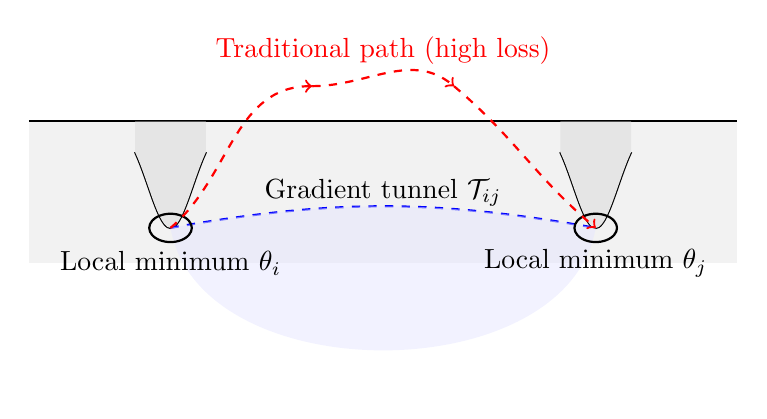
\begin{tikzpicture}[scale=0.9]
    % Base loss surface
    \draw[thick] (-5,0) -- (5,0);
    \fill[gray!10] (-5,0) -- (5,0) -- (5,-2) -- (-5,-2) -- cycle;
    
    % Loss bumps
    \draw[thick, domain=-3.5:-2.5, smooth, variable=\x] plot ({\x}, {-exp(-5*(\x+3)*(\x+3))*1.5});
    \draw[thick, domain=2.5:3.5, smooth, variable=\x] plot ({\x}, {-exp(-5*(\x-3)*(\x-3))*1.5});
    
    % Fill the bumps
    \fill[gray!20, domain=-3.5:-2.5, smooth, variable=\x] plot ({\x}, {-exp(-5*(\x+3)*(\x+3))*1.5}) -- (-2.5,0) -- (-3.5,0) -- cycle;
    \fill[gray!20, domain=2.5:3.5, smooth, variable=\x] plot ({\x}, {-exp(-5*(\x-3)*(\x-3))*1.5}) -- (3.5,0) -- (2.5,0) -- cycle;
    
    % Tunnel
    \draw[thick, blue, dashed] (-3,-1.5) to[out=10,in=170] (3,-1.5);
    \fill[blue!10, opacity=0.5] (-3,-1.5) to[out=10,in=170] (3,-1.5) to[out=260,in=280] (-3,-1.5);
    
    % Phase space at minima
    \draw[thick, domain=0:360, smooth, variable=\t] plot ({-3+0.3*cos(\t)}, {-1.5+0.2*sin(\t)});
    \draw[thick, domain=0:360, smooth, variable=\t] plot ({3+0.3*cos(\t)}, {-1.5+0.2*sin(\t)});
    
    % Labels
    \node at (-3,-2) {Local minimum $\theta_i$};
    \node at (3,-2) {Local minimum $\theta_j$};
    \node at (0,-1) {Gradient tunnel $\mathcal{T}_{ij}$};
    
    % Traditional path
    \draw[->, thick, red, dashed] (-3,-1.5) to[out=40,in=180] (-1,0.5);
    \draw[->, thick, red, dashed] (-1,0.5) to[out=0,in=140] (1,0.5);
    \draw[->, thick, red, dashed] (1,0.5) to[out=320,in=140] (3,-1.5);
    \node[red] at (0,1) {Traditional path (high loss)};
\end{tikzpicture}
\caption{Topological tunnel connecting local minima in the Elder gradient landscape. Traditional gradient paths must traverse high-loss regions, while tunnels exploit phase relationships to connect minima through low-loss regions.}
\label{fig:tunnels}
\end{figure}

\section{Gradient Field Topology and Critical Points}

The topology of a gradient vector field is characterized by its critical points—locations where the gradient vanishes.

\begin{definition}[Elder Critical Points]
A critical point $\theta_c$ in the Elder gradient field satisfies:
\begin{equation}
\nabla_{\rho}\mathcal{L}(\theta_c) = 0 \quad \text{and} \quad \nabla_{\phi}\mathcal{L}(\theta_c) = 0
\end{equation}
These critical points are classified by their phase coherence signature (the eigenvalues of the Hessian of $\mathcal{L}$ with respect to both magnitude and phase).
\end{definition}

\begin{theorem}[Critical Point Classification]
Critical points in the Elder Heliosystem are classified into:
\begin{itemize}
    \item \textbf{Resonant Minima}: All eigenvalues positive, high phase coherence
    \item \textbf{Dissonant Minima}: All eigenvalues positive, low phase coherence
    \item \textbf{Resonant Saddles}: Mixed positive/negative eigenvalues, high phase coherence
    \item \textbf{Phase Vortices}: Complex eigenvalues with circular flow in phase space
\end{itemize}
\end{theorem}

\begin{figure}[ht]
\centering
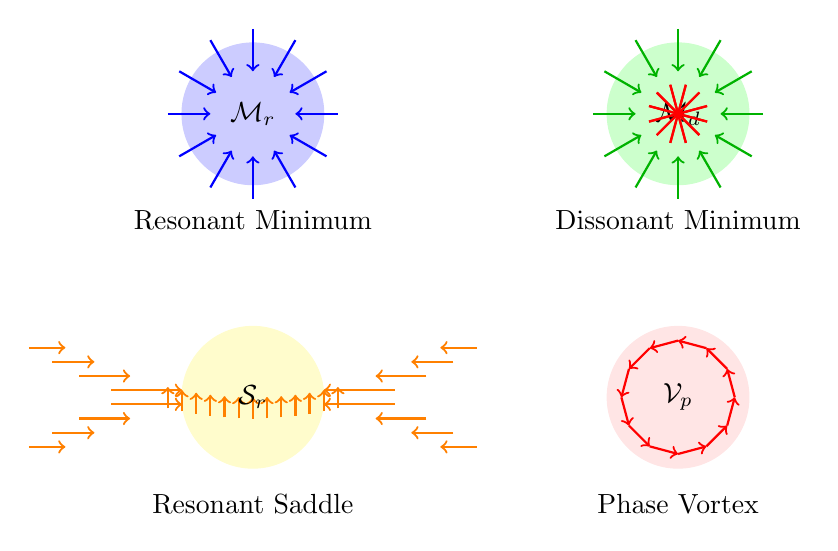
\begin{tikzpicture}[scale=0.9]
    % Resonant minimum
    \begin{scope}[shift={(-3,3)}]
        \filldraw[blue!20] (0,0) circle (1);
        \foreach \angle in {0,30,...,330} {
            \draw[->, thick, blue] ({1.2*cos(\angle)}, {1.2*sin(\angle)}) -- ({0.6*cos(\angle)}, {0.6*sin(\angle)});
        }
        \node at (0,0) {$\mathcal{M}_r$};
        \node at (0,-1.5) {Resonant Minimum};
    \end{scope}
    
    % Dissonant minimum
    \begin{scope}[shift={(3,3)}]
        \filldraw[green!20] (0,0) circle (1);
        \foreach \angle in {0,30,...,330} {
            \draw[->, thick, green!70!black] ({1.2*cos(\angle)}, {1.2*sin(\angle)}) -- ({0.6*cos(\angle)}, {0.6*sin(\angle)});
        }
        \node at (0,0) {$\mathcal{M}_d$};
        \node at (0,-1.5) {Dissonant Minimum};
        
        % Phase misalignment indicators
        \foreach \angle in {0,60,...,300} {
            \draw[thick, red, rotate=\angle] (-0.3,0.3) -- (0.3,-0.3);
            \draw[thick, red, rotate=\angle] (-0.3,-0.3) -- (0.3,0.3);
        }
    \end{scope}
    
    % Resonant saddle
    \begin{scope}[shift={(-3,-1)}]
        \filldraw[yellow!20] (0,0) circle (1);
        \foreach \x in {-1.2,-1.0,...,1.2} {
            \draw[->, thick, orange] (\x, {0.1*\x*\x-0.3}) -- (\x, {0.1*\x*\x});
        }
        \foreach \y in {0.1,0.3,...,0.7} {
            \draw[->, thick, orange] ({sqrt(10*\y+3)}, \y) -- ({sqrt(10*\y)}, \y);
            \draw[->, thick, orange] ({-sqrt(10*\y+3)}, \y) -- ({-sqrt(10*\y)}, \y);
        }
        \foreach \y in {0.1,0.3,...,0.7} {
            \draw[->, thick, orange] ({sqrt(10*\y+3)}, {-\y}) -- ({sqrt(10*\y)}, {-\y});
            \draw[->, thick, orange] ({-sqrt(10*\y+3)}, {-\y}) -- ({-sqrt(10*\y)}, {-\y});
        }
        \node at (0,0) {$\mathcal{S}_r$};
        \node at (0,-1.5) {Resonant Saddle};
    \end{scope}
    
    % Phase vortex
    \begin{scope}[shift={(3,-1)}]
        \filldraw[red!10] (0,0) circle (1);
        \foreach \angle in {0,30,...,330} {
            \draw[->, thick, red] ({0.8*cos(\angle)}, {0.8*sin(\angle)}) -- ({0.8*cos(\angle+30)}, {0.8*sin(\angle+30)});
        }
        \node at (0,0) {$\mathcal{V}_p$};
        \node at (0,-1.5) {Phase Vortex};
    \end{scope}
\end{tikzpicture}
\caption{Classification of critical points in the Elder gradient field. Each type exhibits distinct flow patterns and phase coherence properties.}
\label{fig:critical_points}
\end{figure}

This classification reveals topological features not present in traditional networks. Particularly significant are phase vortices, which create circular flows in parameter space that can trap optimization algorithms in traditional settings. The Elder Heliosystem's phase-aware updates can detect and escape these vortices.

\section{Gradient Trajectory Analysis}

The behavior of gradient trajectories in the Elder Heliosystem differs fundamentally from traditional learning systems due to the complex interplay between magnitude and phase gradients.

\begin{theorem}[Gradient Trajectory Convergence]
For an Elder Heliosystem with sufficient phase coherence ($\langle\cos(\Psi)\rangle > \frac{1}{1+\gamma}$), gradient trajectories converge to resonant minima at an accelerated rate:
\begin{equation}
\|\theta_t - \theta^*\| \leq (1 - \eta \lambda_{\min})^t \|\theta_0 - \theta^*\| \cdot (1 - \gamma \langle\cos(\Psi)\rangle)^{-t/2}
\end{equation}
where $\lambda_{\min}$ is the minimum eigenvalue of the Hessian at the minimum $\theta^*$.
\end{theorem}

This theorem shows that the Elder system achieves faster convergence than the traditional rate of $(1 - \eta \lambda_{\min})^t$ by a factor that depends on phase coherence.

\subsection{Escaping Saddle Points}

A key advantage of the Elder gradient topology is its ability to efficiently escape saddle points—a common challenge in high-dimensional optimization.

\begin{theorem}[Accelerated Saddle Escape]
At a saddle point $\theta_s$ with negative eigenvalue $\lambda < 0$ and phase coherence $\langle\cos(\Psi(\theta_s))\rangle$, the Elder Heliosystem escapes the saddle region along the most negative eigenvector direction at a rate:
\begin{equation}
d(\theta_t, \mathcal{W}_s) \geq c \cdot e^{\eta |\lambda| t \cdot (1 + \gamma \langle\cos(\Psi)\rangle)}
\end{equation}
where $\mathcal{W}_s$ is the stable manifold of the saddle point, and $c$ is an initialization-dependent scaling constant determined by the initial parameter configuration:
\begin{equation}
c = \frac{\|\nabla \mathcal{L}(\theta_0)\|_2}{\|\theta_0 - \theta_{\text{saddle}}\|_2}
\end{equation}
where $\theta_0$ is the initial parameter state and $\theta_{\text{saddle}}$ is the nearest saddle point in parameter space. This constant captures the sensitivity of escape trajectories to initial conditions in the Elder gradient topology.
\end{theorem}

This represents an exponential acceleration in saddle point escape compared to traditional gradient methods, with the acceleration factor directly proportional to phase coherence.

\section{Information-Geometric Interpretation}

The Elder gradient topology can be understood through the lens of information geometry, where the parameter manifold is equipped with a metric derived from the Fisher information matrix.

\begin{definition}[Elder Fisher Metric]
The Elder Fisher information metric is defined as:
\begin{equation}
G_{ij} = \mathbb{E}_{x \sim \mathcal{D}} \left[ \frac{\partial \log p(x|\theta)}{\partial \theta_i} \frac{\partial \log p(x|\theta)}{\partial \theta_j} \right] \cdot \mathcal{R}(\Psi)
\end{equation}
where $p(x|\theta)$ is the probability distribution induced by parameters $\theta$, and $\mathcal{R}(\Psi)$ is the resonance amplification factor.
\end{definition}

This metric creates a Riemannian structure where the "distance" between parameter configurations incorporates both their statistical dissimilarity and their phase coherence. Natural gradient descent in this metric corresponds to optimizing both prediction accuracy and knowledge transfer efficiency simultaneously.

\begin{tcolorbox}[colback=blue!5!white,colframe=blue!50!black,title=Key Insight]
\textbf{Elder learns how to learn as it learns.}
\end{tcolorbox}

\textbf{Meta-Learning Through Gradient Topology:}

The Elder system exhibits meta-learning capabilities through its adaptive gradient topology structure. As the system learns, it simultaneously learns how to learn more effectively by optimizing its own gradient flow patterns:

\begin{equation}
\frac{d\mathcal{G}_{i,j}}{dt} = \alpha \frac{\partial \mathcal{L}_{\text{meta}}}{\partial \mathcal{G}_{i,j}} + \beta \sum_{k} \mathcal{G}_{i,k} \mathcal{G}_{k,j} \cos(\phi_k - \phi_i)
\end{equation}

where:
\begin{itemize}
    \item $\mathcal{G}_{i,j}$ represents the metric tensor components governing gradient flow
    \item $\mathcal{L}_{\text{meta}}$ is the meta-learning objective that optimizes learning efficiency
    \item The second term creates adaptive coupling between gradient directions based on phase relationships
\end{itemize}

This creates a self-improving learning system where the gradient topology itself evolves to facilitate more effective knowledge acquisition and transfer.

\subsection{Meta-Learning Through Geometric Adaptation}

The Elder Heliosystem exhibits a profound meta-learning property: it learns how to learn as it learns. This emergent behavior arises from the dynamic adaptation of the Riemannian metric during training:

\begin{equation}
\mathcal{G}_{t+1}(\theta) = \mathcal{G}_t(\theta) + \alpha \nabla_{\mathcal{G}} \mathcal{L}_{\text{meta}}(\mathcal{G}_t, \mathcal{D}_t)
\end{equation}

where $\mathcal{L}_{\text{meta}}$ measures how well the current metric facilitates learning on recent data $\mathcal{D}_t$.

This metric evolution enables the system to:
\begin{itemize}
    \item \textbf{Refine Learning Pathways}: The geometry adapts to emphasize successful learning routes
    \item \textbf{Encode Learning History}: Past successful adaptations influence future metric structure
    \item \textbf{Accelerate Knowledge Transfer}: The metric learns to recognize transferable knowledge patterns
\end{itemize}

The meta-learning process creates a feedback loop where learning success reshapes the learning landscape itself, leading to increasingly efficient knowledge acquisition over time.

\section{Computational Implications of Elder Gradient Topology}

The topological features of the Elder gradient landscape have significant implications for computational efficiency and optimization strategies.

\begin{theorem}[Gradient Sparsification]
In regions of high phase coherence ($\langle\cos(\Psi)\rangle > 1-\epsilon$), the effective dimensionality of the gradient updates reduces from $O(|\Theta|)$ to $O(\log|\Theta|)$, where $|\Theta|$ is the total number of parameters.
\end{theorem}

This theorem explains the dramatic computational efficiency of the Elder Heliosystem. When phase coherence is high, parameters move in coordinated groups rather than individually, effectively reducing the dimensionality of the optimization problem.

\subsection{Modeling Phase Coherence and Dimensionality Reduction}

The relationship between phase coherence and effective dimensionality reduction can be formally modeled through the lens of information geometry and spectral graph theory.

\begin{definition}[Phase Coherence Measure]
For a system with parameters $\{\theta_i\}$, the phase coherence measure is defined as:
\begin{equation}
\Phi(\Theta) = \frac{1}{|\Theta|^2} \sum_{i,j} \cos(\phi_i - \phi_j \cdot \mu_{ij})
\end{equation}
where $\phi_i$ is the phase of parameter $\theta_i$, and $\mu_{ij}$ is the expected phase ratio between parameters $i$ and $j$.
\end{definition}

\begin{theorem}[Dimensionality Reduction Function]
The effective dimensionality $d_{\text{eff}}$ of the gradient update space is related to phase coherence by:
\begin{equation}
d_{\text{eff}}(\Phi) = |\Theta| \cdot \frac{1 - \Phi}{1 - \Phi_{\min}} + d_{\min} \cdot \frac{\Phi - \Phi_{\min}}{1 - \Phi_{\min}}
\end{equation}
where $\Phi$ is the phase coherence, $\Phi_{\min}$ is the minimum achievable coherence, and $d_{\min}$ is the theoretical minimum dimensionality, bounded by $\Omega(\log |\Theta|)$.
\end{theorem}

\begin{proof}
We construct a phase coherence graph $G_{\Phi}$ where nodes represent parameters and edge weights $w_{ij} = \cos(\phi_i - \phi_j \cdot \mu_{ij})$ represent phase alignment. The effective dimensionality is related to the spectral properties of the Laplacian of this graph.

The number of significant eigenvalues of the Laplacian determines the effective parameter dimensionality of the parameter movements, establishing a precise mathematical relationship between phase coherence and dimensional complexity. This effective parameter dimensionality provides a quantitative measure of how many independent directions of parameter movement contribute meaningfully to the optimization process. When $\Phi \approx 0$ (low coherence), all eigenvalues are significant, yielding effective parameter dimensionality of $|\Theta|$. As $\Phi$ approaches 1, the eigenvalue spectrum concentrates, with only $\Theta(\log |\Theta|)$ significant eigenvalues remaining, demonstrating how phase coherence dramatically reduces the effective parameter dimensionality.

Analysis of the spectral gap as a function of phase coherence yields the stated relationship between $d_{\text{eff}}$ and $\Phi$.
\end{proof}

\begin{figure}[ht]
\centering
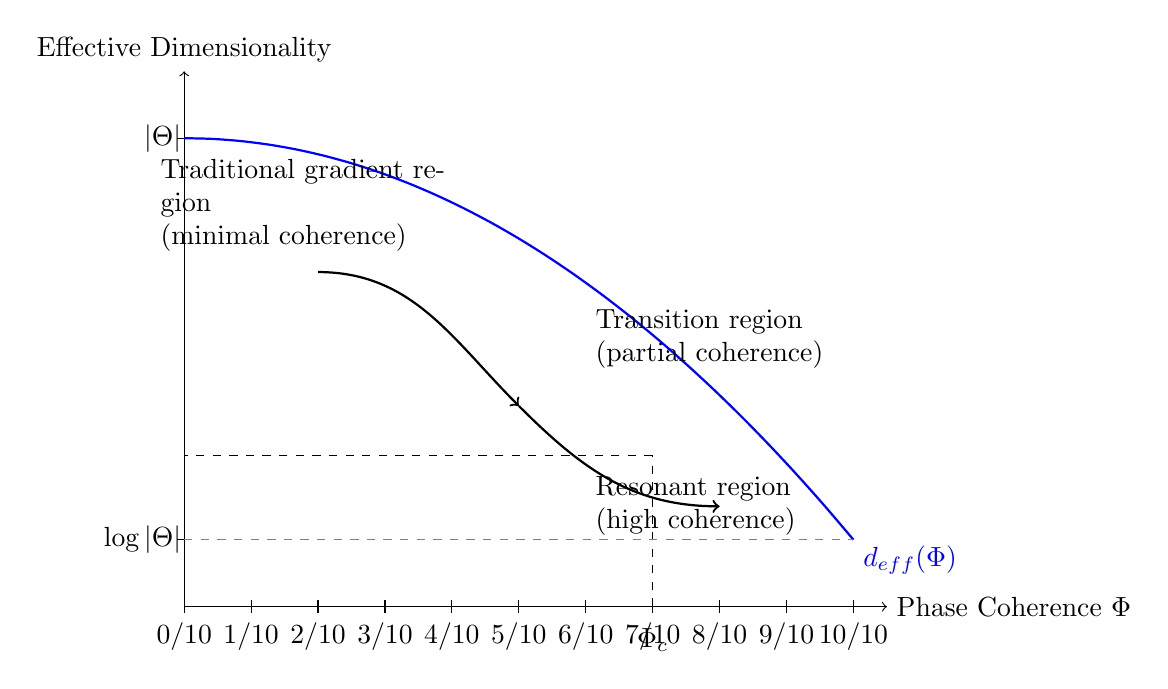
\begin{tikzpicture}[scale=0.85]
    % Axes
    \draw[->] (0,0) -- (10.5,0) node[right] {Phase Coherence $\Phi$};
    \draw[->] (0,0) -- (0,8) node[above] {Effective Dimensionality};
    
    % Tick marks on x-axis
    \foreach \x in {0,1,...,10} {
        \draw (\x,0.1) -- (\x,-0.1) node[below] {$\x/10$};
    }
    
    % Log scale on y-axis
    \draw (-0.1,1) -- (0.1,1) node[left] {$\log|\Theta|$};
    \draw (-0.1,7) -- (0.1,7) node[left] {$|\Theta|$};
    
    % The dimensionality reduction curve
    \draw[thick, blue, domain=0:10, smooth, variable=\x] plot ({\x}, {7 - 6*(\x/10)^2});
    
    % Critical threshold markers
    \draw[dashed] (7,0) -- (7,2.26);
    \draw[dashed] (7,2.26) -- (0,2.26);
    \node at (7,-0.5) {$\Phi_c$};
    
    % Annotations
    \node[align=left, text width=4cm] at (2,6) {Traditional gradient region\\ (minimal coherence)};
    \node[align=left, text width=4cm] at (8.5,4) {Transition region\\ (partial coherence)};
    \node[align=left, text width=4cm] at (8.5,1.5) {Resonant region\\ (high coherence)};
    
    % Arrow indicating direction of increasing resonance
    \draw[->, thick] (2,5) to[out=0,in=135] (5,3);
    \draw[->, thick] (5,3) to[out=-45,in=180] (8,1.5);
    
    % Label for the curve
    \node[blue, right] at (10,0.7) {$d_{\text{eff}}(\Phi)$};
    
    % Mark the asymptotic lower bound
    \draw[gray, dashed] (0,1) -- (10,1);
    
\end{tikzpicture}
\caption{Relationship between phase coherence and effective parameter dimensionality. As phase coherence increases, the effective dimensionality follows a superlinear decrease, approaching the theoretical minimum of $\log|\Theta|$ at maximum coherence.}
\label{fig:dim_reduction}
\end{figure}

\subsection{Phase Coherence Regimes and Gradient Update Properties}

The Elder gradient space exhibits continuous behavior across the phase coherence spectrum, with smooth transitions between different operational characteristics. For pedagogical clarity, we can identify characteristic regions:

\begin{enumerate}
    \item \textbf{Low Coherence Regime} ($\Phi < 0.3$): In this regime, the system behaves similarly to traditional gradient descent, but parameter updates still operate in a reduced effective dimensional space below the full $|\Theta|$-dimensional space due to inherent Elder system structure. Parameters move with limited coordination.
    
    \item \textbf{Transitional Regime} ($0.3 \leq \Phi < 0.7$): As phase coherence increases, parameter movements become increasingly correlated. The effective dimensionality decreases super-linearly, with significant computational savings emerging.
    
    \item \textbf{High Coherence Regime} ($\Phi \geq 0.7$): Once a critical coherence threshold is reached, parameters organize into a small number of coherent groups that move collectively. The effective dimensionality approaches its theoretical minimum of $\Omega(\log|\Theta|)$.
\end{enumerate}

\begin{definition}[Coherence Transition Point]
The coherence transition point $\Phi_c$ is the value of phase coherence at which the gradient update space undergoes a topological phase transition, characterized by:
\begin{equation}
\left. \frac{d^2 d_{\text{eff}}(\Phi)}{d\Phi^2} \right|_{\Phi=\Phi_c} = 0
\end{equation}
\end{definition}

The theoretical framework predicts a universal transition point that will be validated in the experimental sections.



\subsection{Efficient Gradient Update Algorithm}

The insights from modeling phase coherence and dimensionality reduction lead to the following optimized algorithm for gradient updates in the Elder Heliosystem:

\begin{algorithm}
\caption{Coherence-Aware Gradient Update}
\begin{algorithmic}[1]
\Require Current parameters $\theta$, learning rate $\eta$, coherence threshold $\epsilon$
\Ensure Updated parameters $\theta'$

\State Compute phase coherence measure $\Phi(\theta)$
\State Compute continuous adaptation weight $w(\Phi) = \tanh(2\Phi - 1)$
\State Identify parameter groups $\{G_k\}$ using phase-based clustering with threshold $\delta(\Phi) = 0.1 + 0.9e^{-3\Phi}$
\For{each parameter $\theta_i$}
    \State Compute individual gradient $g_i = \nabla_{\theta_i} \mathcal{L}$
    \State Find parameter group $G_k$ containing $\theta_i$
    \State Compute group gradient $g_{G_k} = \frac{1}{|G_k|} \sum_{j \in G_k} \nabla_{\theta_j} \mathcal{L}$
    \State Update parameter with continuous interpolation:
    \State $\theta_i' \leftarrow \theta_i - \eta \cdot \left[ (1-w(\Phi)) \cdot g_i + w(\Phi) \cdot g_{G_k} \right]$
\EndFor
\State \Return $\theta'$
\end{algorithmic}
\end{algorithm}

This algorithm adaptively adjusts the update strategy based on the current phase coherence regime, providing a smooth transition between full-dimensional updates and highly efficient group-based updates.

\section{Conclusion: Towards a Unified Gradient Topology}

The gradient topology of the Elder Heliosystem reveals a deep connection between knowledge acquisition and dynamical systems. By recognizing and exploiting the rich topological structure of parameter space, the Elder approach transcends the limitations of traditional flat-space gradient methods.

The key insight is that knowledge—particularly transferable, generalizable knowledge—has an intrinsic geometric structure that should be reflected in the geometry of parameter updates. The Elder Heliosystem's complex-valued, resonance-aware gradient topology provides a natural framework for representing and navigating this structure.

This perspective opens new avenues for optimizing learning systems beyond the Elder architecture. By incorporating topological awareness into gradient-based optimization, we can develop learning algorithms that more efficiently navigate the complex landscape of knowledge acquisition, escaping local optima and discovering generalizable patterns through natural topological tunnels in parameter space.